\documentclass[conference]{IEEEtran}
\usepackage{blindtext, graphicx}

\usepackage[slovak]{babel}
\usepackage[utf8]{inputenc}
\usepackage{cite}

\usepackage{url}
\usepackage{amsmath}

\usepackage{algorithm}
\usepackage{algpseudocode}

\algnewcommand\algorithmicforeach{\textbf{for each}}
\algdef{S}[FOR]{ForEach}[1]{\algorithmicforeach\ #1\ \algorithmicdo}

% correct bad hyphenation here
\hyphenation{op-tical net-works semi-conduc-tor}

\begin{document}
%
% paper title
% can use linebreaks \\ within to get better formatting as desired
\title{Porovnanie času konvergencie siete medzi softvérovo riadenými sieťami a sieťami podporujúcimi protokol OSPF}

% author names and affiliations
% use a multiple column layout for up to three different
% affiliations
\author{\IEEEauthorblockN{Peter Kaňuch}
\IEEEauthorblockA{Fakulta informatiky a informačných technológií\\
Slovenská Technická Univerzita\\
Slovenská republika, 841 04 Bratislava IV\\
Email: xkanuch@stuba.sk}\and
\IEEEauthorblockN{Nikolas Janec}
\IEEEauthorblockA{Fakulta informatiky a informačných technológií\\
Slovenská Technická Univerzita\\
Slovenská republika, 841 04 Bratislava IV\\
Email: xjanec@stuba.sk}}



% use for special paper notices
%\IEEEspecialpapernotice{(Invited Paper)}

% make the title area
\maketitle

\begin{abstract}
%\boldmath
Dynamické smerovacie protokoly sa v posledných desaťročiach značne rozvinuli. Avšak pri súčasných narastajúcich požiadavkách sa ich zavedenie do vnútorných firemných sieti stáva nevhodné v mnohých aspektoch. Ako východiskom pri súčasných požiadavkách sa stáva aplikovanie softvérovo definovaných sietí – SDN. Tento článok bol vypracovaný za účelom porovnania dosiahnutých výsledkov práce opísanych v článku  \cite{article}, kde autori porovnávali časy konvergencie a doby odozvy medzi OSPF ako zástupcom dynamických smerovacích protokolov a SDN. Naše výsledky potvrdili, že nasadenie SDN je v súčasnosti lepšou alternatívou ako OSPF. Ale výsledné časy neboli až tak rozdielne ako je uvedené v danom článku.
\end{abstract}

\begin{IEEEkeywords}
SDN, Mininet, OpenFlow, HP Van, OSPF, Cisco iOS
\end{IEEEkeywords}

\IEEEpeerreviewmaketitle

\section{Úvod}

Najčastejšie používaným smerovacím protokolom vo veľkých korporátnych, či firemných sieťach je protokol OSPF (\textit{Open Shortest Path First}) z dôvodu, že tento protokol podporuje širokú škálu funkcionality pre siete poskytovateľov \cite{first}. V poslednom období sa začali dostávať do popredia SDN siete (\textit{Softvérovo riadené siete}), ktoré prinášajú určité výhody oproti klasickým sieťam.

\section{OSPF}

Je dynamický smerovací protokol, ktorý sa používa v rámci jedného autonómneho systému (IGP). Patrí do skupiny Link-state protokolov vďaka čomu smerovač vo firemnej sieti pozná:

\begin{itemize}
	\item{Všetky ostatné smerovače}
	\item{Vzájomné prepojenia medzi smerovačmi}
	\item{Všetky koncové aj prepojovacie siete}
	\item{Ceny všetkých rozhraní}
\end{itemize}

OSPF sa skladá z troch štruktúr:

\begin{enumerate}
\item{Tabuľka susedov – informácie o známych susedov}
\item{Topologická databáza – informácie o všetkých smerovačoch a ich pripojených sieťach v danej oblasti ale taktiež aj informácie o sieťach v iných oblastiach, nad touto databázou každý smerovač pomocou SPF algoritmu si prepočíta najkratšiu cestu ku všetkým uzlom v sieti}
\item{Smerovacia tabuľka – obsahuje next-hop na najkratšu cestu pre každú známu sieť}\cite{ospf}
\end{enumerate}

\section{Softvérovo riadené siete}

\subsection{SDN}
Softvérovo riadené siete (SDN) majú centralizovanú architektúru \cite{second}, čo znamená, že zariadenia v sieti sú centralizovane riadené z jedného kontroléra. SDN architektúru tvoria nasledovné vrstvy:

\begin{itemize}
	\item{Aplikačná vrstva - ponúka služby pre virtualizáciu, smerovanie, firewall, ...}
	\item{Kontrolná vrstva - pozostáva z kontrolera, ktorý jednak komunikuje s aplikáciami cez rozhranie, ale aj priamo s fyzickou vrstvou (infraštruktúrou).}
	\item{Vrstva infraštruktúry - pozostáva z fyzických zariadení pripojených v sieti}
\end{itemize}

Základným prvkom v Softvérovo riadených sieťach je virtualizácia. Tá dovoľuje, aby softvér, ktorý riadi celú sieť bežal nezávisle od fyzickej vrstvy (zariadení/hardvéru) \cite{third}.

\begin{figure}[h!]
\centering
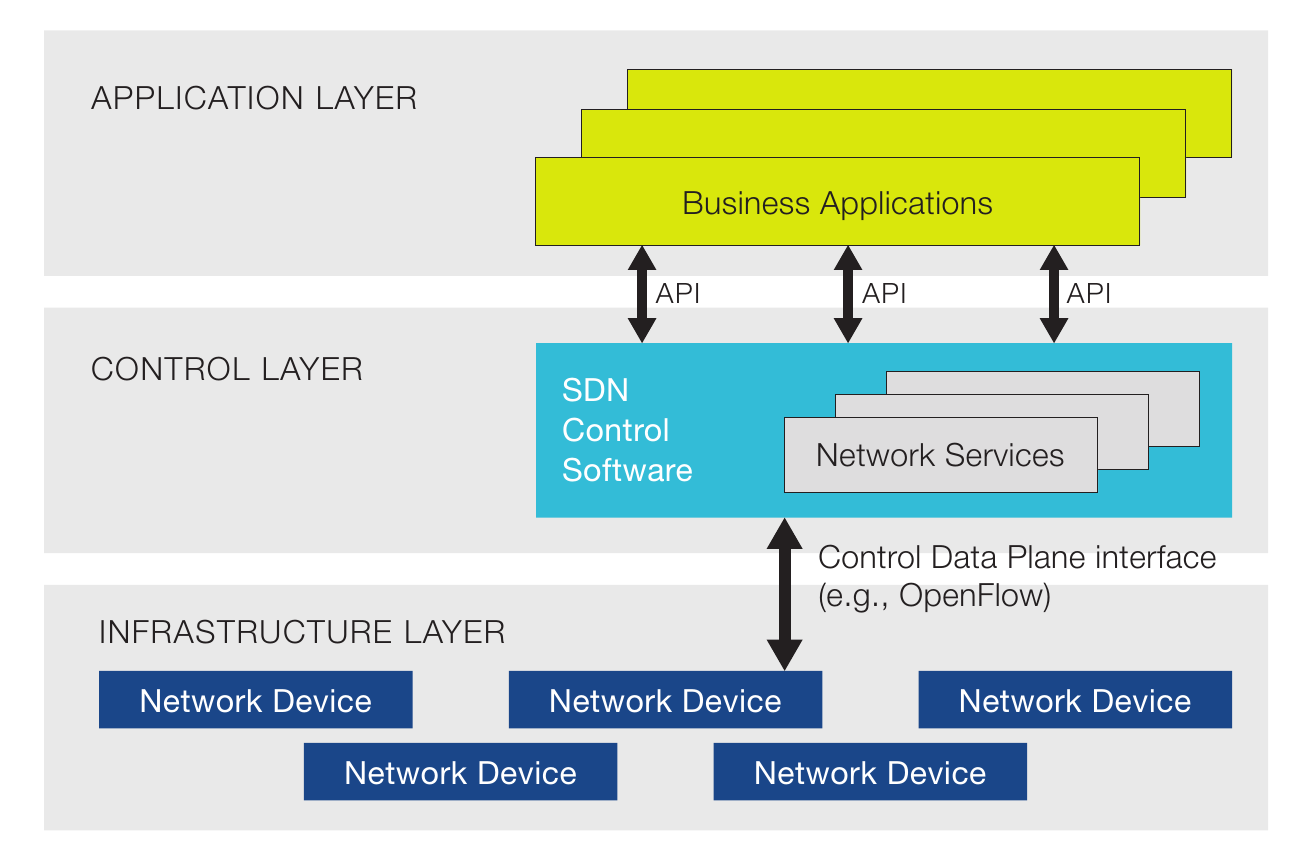
\includegraphics[width=3in]{../img/sdn-architecture}
\caption{SDN architektúra}
\end{figure}

\subsection{OpenFlow}

Komunikačný protokol pre SDN siete, ktorý umožňuje priamu interakciu kontrolera s fyzickými zariadeniami. Je štandard, ktorý dovoľuje vzdialene konfigurovať zariadenia od rôznych výrobcov \cite{fourth}. Taktiež umožňuje úpravu smerovacích tabuliek pomocou pridávania rôznych pravidiel.

\section{Testovanie}

\subsection{Testovacie prostredie}

\begin{itemize}
\item{VirtualBox v5.1.28}
\item{Ubuntu-14.04.5-server-amd64}
\item{Mininet simulátor -}
Mininet je nástroj určený pre simuláciu SDN sieti \cite{fifth}. Napodobňuje kompletnú sieť zariadení ako hosty, prepínače a jednotlivé prepojenia medzi nimi. Dokáže simulovať sieť pomocou virtualizácie založeniej na procesoch. Taktiež podporuje protokol OpenFlow.
\item{HP Van SDN kontrolér 2.7.18 -} je softvér, ktorý poskytuje centrálny bod pre správu sieti podporujúce protokol OpenFlow \cite{sixth}. Taktiež poskytuje rozhranie pre vývoj Java aplikácií inými vývojarmi. Je navrhnutý najmä pre fungovanie v dátových centrách. Návod na jeho inštaláciu a potrebné nastavenia nájdete na \url{github.com} k tomuto článku.

\begin{figure}[h!]
\centering
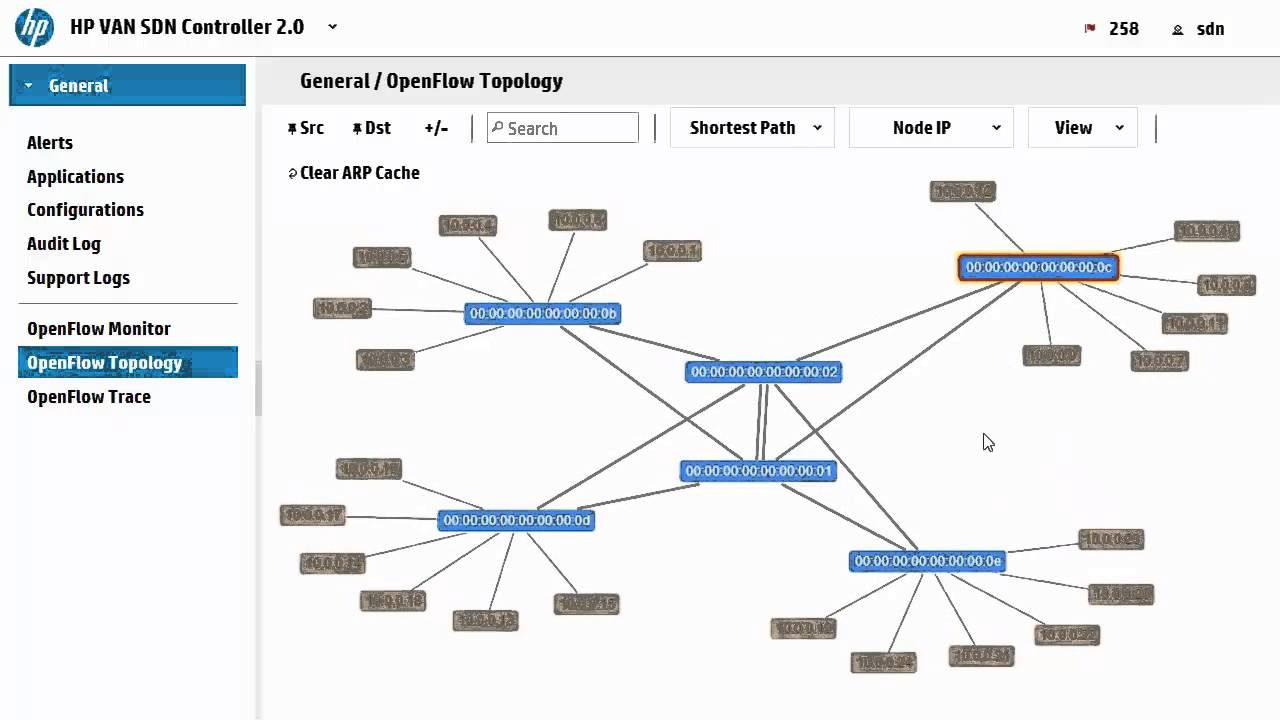
\includegraphics[width=3in]{../img/HPVAN}
\caption{HP Van SDN kontrolér}
\end{figure}


\item{Python}
\item{Cisco iOS 7200}
\item{GNS3 -} nástroj určený pre simuláciu sieti podporujúcich Cisco zariadenia.
\item{TCPping -} nástroj, ktorý dokáže simulovať HTTP komunikáciu.
\end{itemize}

\subsection{Topológia siete \label{topo}}

Pre testovacie účely sme vytvorili tri veľkostí topológie, a to topológia s desiatimi, dvadsiatimi a tridsiatimi zariadeniami. V topológii sú na oboch jej koncoch zapojené počítače. Každá linka v sieti medzi dvoma zariadeniami má nasledujúce parametre:

\begin{enumerate}
\item{bandwidth linky = 10}
\item{delay = 1.5 ms}
\item{spoľahlivosť (loss) = 0}
\end{enumerate}

\begin{figure}[h!]
\centering
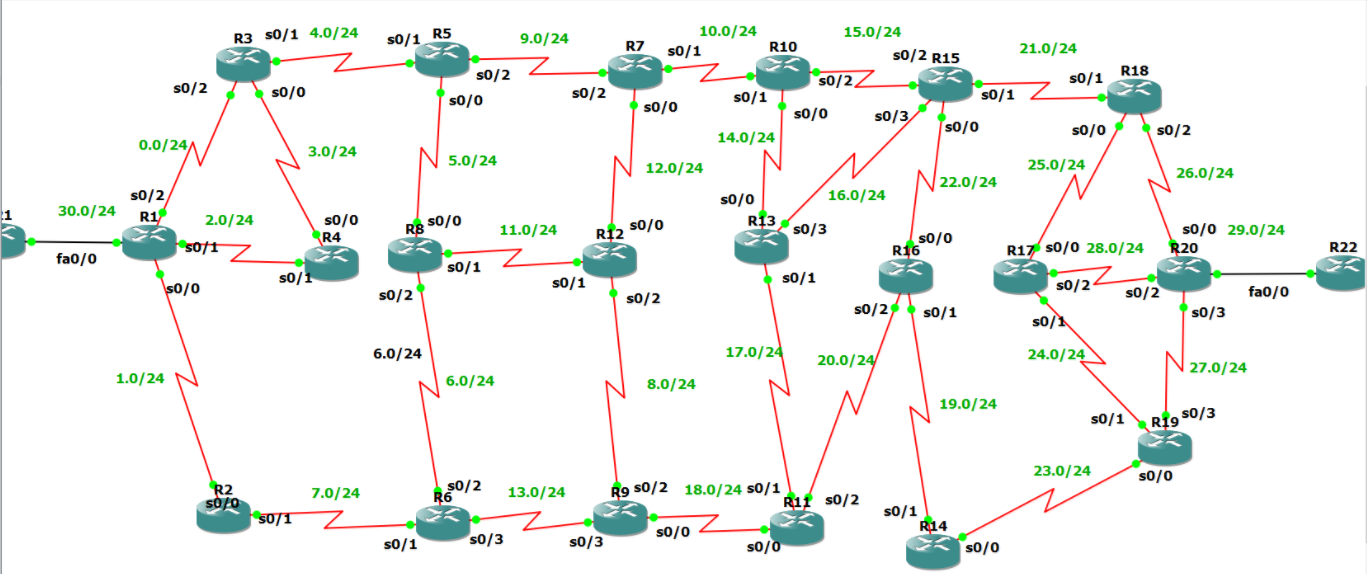
\includegraphics[width=3in]{../img/topology}
\caption{Príklad topológie s dvadsiatimi zariadeniami v nástroji GNS3}
\end{figure}

\begin{figure}[h!]
\centering
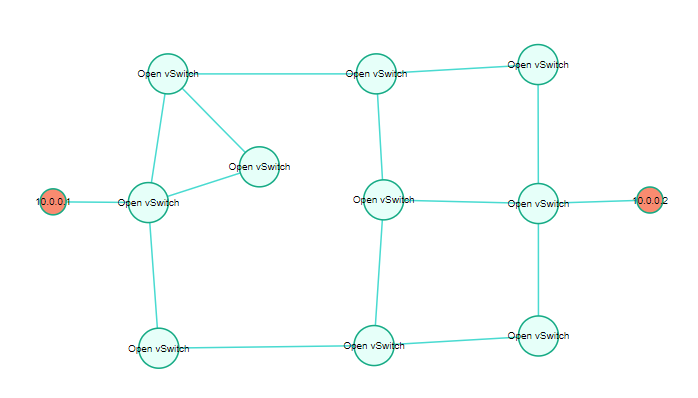
\includegraphics[width=3in]{../img/topologySDN}
\caption{Príklad topológie s desiatimi zariadeniami v Mininete}
\end{figure}

\subsection{Konvergencia siete}

Jednou z charakteristických vecí dynamických smerovacích protokolov je aj to, že sa musia v čo najkratšom možnom čase prispôsobiť na akúkoľvek zmenu v sieti. Smerovací protokol OSPF si pamätá celú topológiu siete a reaguje na akúkoľvek zmenu v sieti, pripojenie/odpojenie linky a pod. Takýto stav, kedy všetky zariadenia v sieti (routre) majú informácie o všetkých linkách a najrýchlejších cestách voláme \textit{konvergencia} a čas, potrebný na dosiahnutie takéhoto stavu po zmene v sieti, nazývame \textit{čas konvergencie} \cite{seventh}.  
Ten v IGP protokoloch pozostáva zo štyroch hlavných častí \cite{eigth}: 

\begin{enumerate}
	\item{Reakcia na zmenu v sieti}
		\begin{itemize}
			\item{Indikačný čas zlyhania/obnovenia na fyzickej vrstve}
			\item{Indikačný čas zlyhania/obnovenia na linkovej vrstve}
			\item{Intervaly časovačov IGP protokolov}
		\end{itemize}
	\item{Čas vykonania algoritmu SPF (Shortest Path First)}
	\item{LSA/LSP oznámenia}
	\item{Čas potrebný na aktualizáciu FIB tabuľky v hardvéri}
\end{enumerate}

Čas konvergencie v SDN sieťach \cite{nineth}:

\begin{enumerate}
	\item{Reakcia na zmenu v sieti}
	\item{Čas potrebný na aktualizáciu topológie}
	\item{Čas vykonania algoritmu SPF (Shortest Path First)}
	\item{Čas potrebný na aktualizáciu Flow tabuľky}
\end{enumerate}

\subsection{Doba odozvy}
Doba odozvy v SDN sieťach pozostáva z:

\begin{enumerate}
	\item{Latencia linky}
	\item{Zhoda vo Flow tabuľke}
	\item{Čas odoslania dát}
\end{enumerate}

Doba odozvy pre OSPF siete pozostáva z:

\begin{enumerate}
	\item{Latencia linky}
	\item{Vyhľadanie v smerovacej tabuľke}
	\item{Čas odoslania dát}
\end{enumerate}

\subsection{Návrh scenára pre testovanie}

Pre odmeranie času konvergencie siete sme navrhli nasledovný scenár:

\begin{itemize}
	\item{Zapojenie navrhnutej topológie z časti \ref{topo}}
	\item{Spustenie HTTP servra na jednom z pripojených hostov do siete}
	\item{Spustenie merania pomocou nástroja TCPping z jedného hosta na host so sputeným HTTP serverom}
	\item{Odpojenie linky v sieti, cez ktorú tečie premávka a tvorí slučku v sieti}
\end{itemize}

Pre uľahčenie vykonávania jednotlivých meraní sme napísali automatické testy naprogramované v pythone pre vykonanie simulácie v prostredí Mininet. 

\section{Výsledky meraní}

V testovacom prostredí sme vykonali 20 meraní pre každú topológiu a dosiahli sme nasledovné výsledky pre čas konvergencie zobrazený v grafoch.

\begin{figure}[h!]
\centering
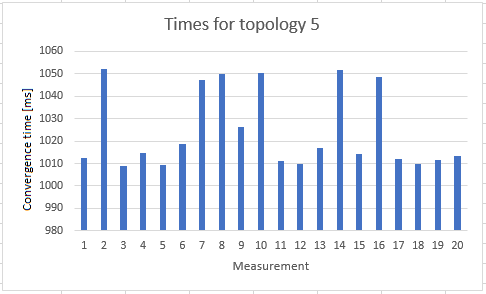
\includegraphics[width=3in]{../img/graph5}
\caption{Čas konvergencie v SDN pre 5 zariadení}
\end{figure}

\begin{figure}[h!]
\centering
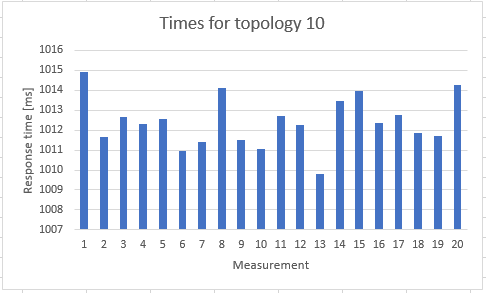
\includegraphics[width=3in]{../img/graph10}
\caption{Čas konvergencie v SDN pre 10 zariadení}
\end{figure}

\begin{figure}[h!]
\centering
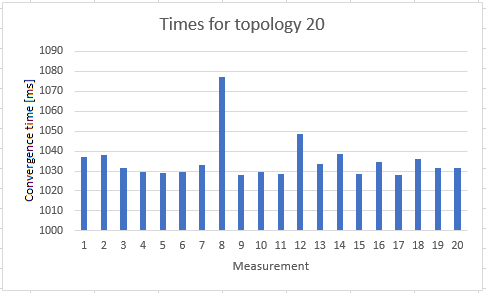
\includegraphics[width=3in]{../img/graph20}
\caption{Čas konvergencie v SDN pre 20 zariadení}
\end{figure}

\begin{figure}[h!]
\centering
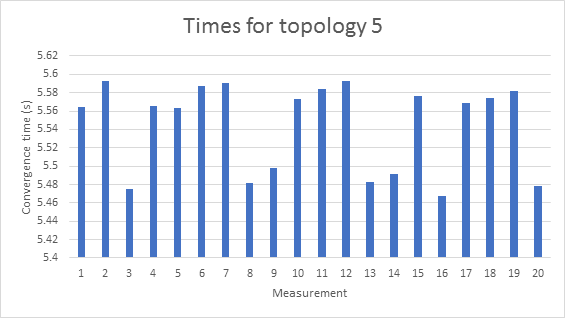
\includegraphics[width=3in]{../img/graph5ospf}
\caption{Čas konvergencie pre OSPF pre 5 zariadení}
\end{figure}

\begin{figure}[h!]
\centering
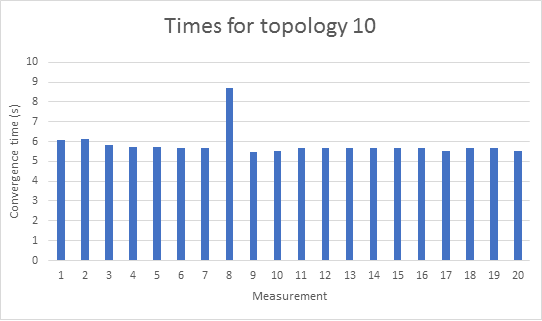
\includegraphics[width=3in]{../img/graph10ospf}
\caption{Čas konvergencie pre OSPF pre 10 zariadení}
\end{figure}

\begin{figure}[h!]
\centering
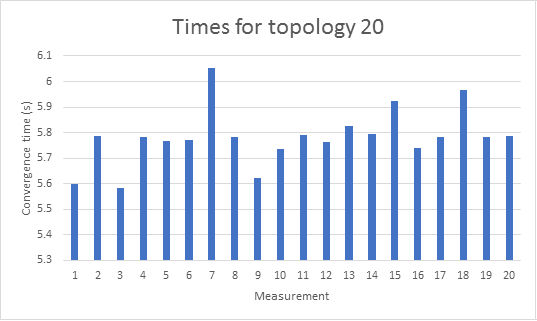
\includegraphics[width=3in]{../img/graph20ospf}
\caption{Čas konvergencie pre OSPF pre 20 zariadení}
\end{figure}

\newpage
V nasledujúcich grafoch sme zobrazili dobu odozvy taktiež pre dané veľkosti topológie. Jednotlivé meranie sme vykonali 20 krát.

\begin{figure}[h!]
\centering
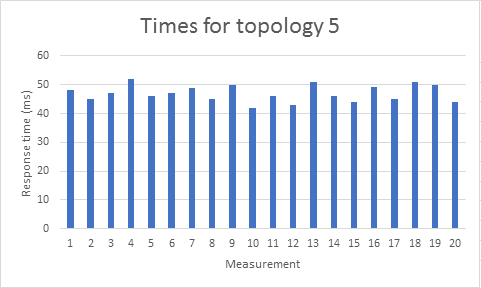
\includegraphics[width=3in]{../img/5responseospf}
\caption{Doba odozvy pre OSPF pre 5 zariadení}
\end{figure}

\begin{figure}[h!]
\centering
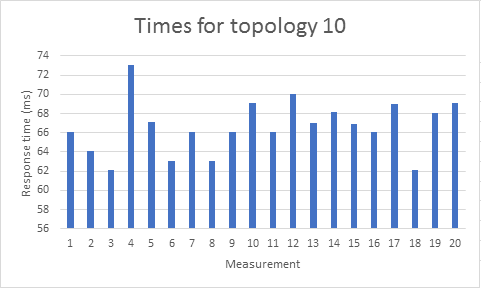
\includegraphics[width=3in]{../img/10responseospf}
\caption{Doba odozvy pre OSPF pre 10 zariadení}
\end{figure}

\begin{figure}[h!]
\centering
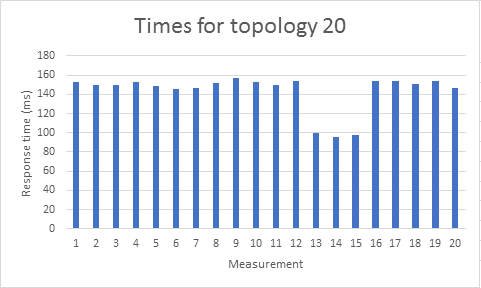
\includegraphics[width=3in]{../img/20responseospf}
\caption{Doba odozvy pre OSPF pre 20 zariadení}
\end{figure}

\begin{figure}[h!]
\centering
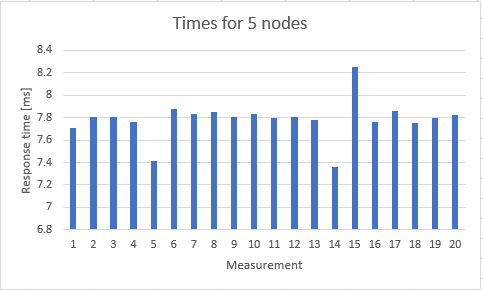
\includegraphics[width=3in]{../img/5responseSDN}
\caption{Doba odozvy v SDN pre 5 zariadení}
\end{figure}

\begin{figure}[h!]
\centering
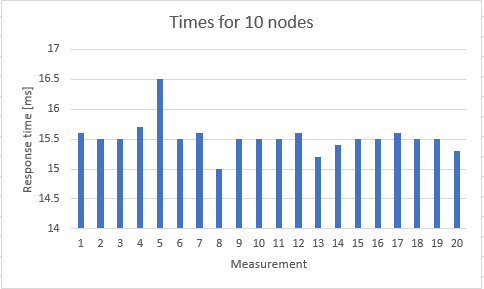
\includegraphics[width=3in]{../img/10responseSDN}
\caption{Doba odozvy v SDN pre 10 zariadení}
\end{figure}

\begin{figure}[h!]
\centering
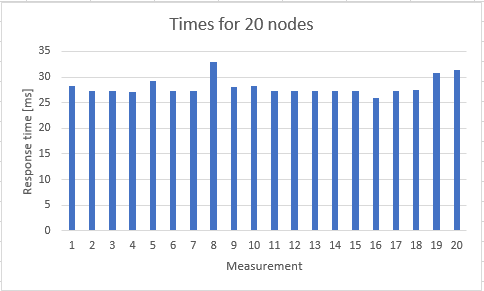
\includegraphics[width=3in]{../img/20responseSDN}
\caption{Doba odozvy v SDN pre 20 zariadení}
\end{figure}


\section{Záver}

V tejto práci sme porovnali časy konvergencie a doby odozvy v sieťach založených na OSPF a SDN s Open vSwitch zariadeniami. Na základe výsledkov môžeme taktiež potvrdiť, že budúcnosťou pri zvyšovaní požiadaviek je práve v aplikovaní SDN. Pri testovaní sme použili rovnaké testovacie prostredie ako autori v článku \cite{article}, no hodnoty boli odlišné. Pri sieťach založených na protokole OSPF nie je možné dosiahnúť tak rozdielne výsledky v časoch konvergencie pri sieťach s 5, 10, 20 uzlami ako uvádzali autori. Taktiež sme nedosiahli rovnaký čas konvergencie v SDN. Autori neuviedli, ktoré linky v sieti boli vypnuté, a preto je možné, že narozdiel od nás, zhodili linku v slučke cez ktorú netiekla premávka. Čo sa týka doby odozvy, taktiež sme dostali iné výsledky, no tie sa približujú viac k výsledkom uvedeným v danom porovnávanom článku.



\begin{table}[h!]
\centering
\caption{Porovnanie priemerných časov doby odozvy a času konvergencie medzi SDN a OSPF sieťami}
\label{my-label}
\begin{tabular}{|c|c|c|c|c|}
\hline
                         & \multicolumn{2}{c|}{\textbf{Čas konvergencie}} & \multicolumn{2}{c|}{\textbf{Doba odozvy}}      \\ \hline
\textbf{Počet zariadení} & \textbf{SDN {[}ms{]}}  & \textbf{OSPF {[}s{]}} & \textbf{SDN {[}ms{]}} & \textbf{OSPF {[}ms{]}} \\ \hline
\textbf{5}               & 1024.47                & 5.54445               & 7.7845                & 47.03885               \\ \hline
\textbf{10}              & 1012.41455             & 5.844                 & 15.525                & 66.60895               \\ \hline
\textbf{20}              & 1035.059               & 5.78175               & 28.1                  & 143.36625              \\ \hline
\end{tabular}
\end{table}





% Can use something like this to put references on a page
% by themselves when using endfloat and the captionsoff option.
\ifCLASSOPTIONcaptionsoff
  \newpage
\fi


\begin{thebibliography}{1}
\bibitem{first}KHAN, Asad Ali, et al. A Convergence Time Optimization Paradigm for OSPF based Networks Through SDN SPF Protocol Computer Communications and Networks (CCN)/Delay Tolerant Networks. In: Proceedings of the International Conference on Future Networks and Distributed Systems. ACM, 2017. p. 43.

\bibitem{second}Software-Defined Networking (SDN) Definition, \url{https://www.opennetworking.org/sdn-definition/}, Accessed: 19.11.2017

\bibitem{third}FOGARTY, Susan. 7 Essentials of Software-Defined Networking. Information Week Network Computing, 2013.

\bibitem{fourth}What is OpenFlow? Definition and How it Relates to SDN, \url{https://www.sdxcentral.com/sdn/definitions/what-is-openflow/},  Accessed: 19.11.2017

\bibitem{fifth}Mininet: Rapid Prototyping for Software Defined Networks, \url{https://github.com/mininet/mininet}

\bibitem{sixth}HP Virtual Application Networks (VAN) SDN Controller, \url{https://www.sdxcentral.com/products/hp-virtual-application-networks-van-sdn-controller/}

\bibitem{seventh}What is Convergence of Routing Tables and What is Convergence Time, \url{http://www.omnisecu.com/cisco-certified-network-associate-ccna/what-is-convergence-of-routing-tables.php},  Accessed: 19.11.2017

\bibitem{eigth}PORETSKY, S.; IMHOFF, B.; MICHIELSEN, K. Benchmarking Methodology for Link-State IGP Data-Plane Route Convergence. 2011.

\bibitem{nineth}ZHANG, Hailong; YAN, Jinyao. Performance of SDN routing in comparison with legacy routing protocols. In: Cyber-Enabled Distributed Computing and Knowledge Discovery (CyberC), 2015 International Conference on. IEEE, 2015. p. 491-494.

\bibitem{article}KHAN, Asad Ali, et al. A Convergence Time Optimization Paradigm for OSPF based Networks Through SDN SPF Protocol Computer Communications and Networks (CCN)/Delay Tolerant Networks. In: Proceedings of the International Conference on Future Networks and Distributed Systems. ACM, 2017. p. 43.

\bibitem{ospf}Ruhann, OSPF Convergence, \url{https://routing-bits.com/2009/08/06/ospf-convergence/}, Accessed: 27.11.2017

\end{thebibliography}






\end{document}


